\chapter{Aufbau}
Abbildung \ref{aufbau} zeigt den physischen Aufbau der Projekts. Auf der einen Seite ist der Raspberry PI erkennbar. Auf der anderen Seite befindet sich ein Arduino UNO, welcher einen Datenlogger darstellen soll. Da zur Zeit der Entwicklung der Datenlogger nicht vorhanden war, wurde mittels eines Arduino UNO dessen Funktionalitäten nachgebaut. Der Arduino UNO zählt die ankommenden Impulse und summiert diese auf. Per Konsole werden die Werte an den Entwickler gegeben, sodass er testen kann, ob die gewünschte Anzahl von Impulsen angekommen ist. Im Betrieb soll jedoch ein richtiger Datenlogger zum Einsatz kommen.\\
Der Kern des Aufbaus bildet der Optokoppler vom Typ KB Knighbright KB 817. Der Optokoppler trennt die beiden Stromkreise voneinander galvanisch. Diese Trennung sichert den Raspberry PI gegen zu hohen Spannungen ab und verhindert somit seine Zerstörung. 
\begin{figure}[H]
 	\centering
 	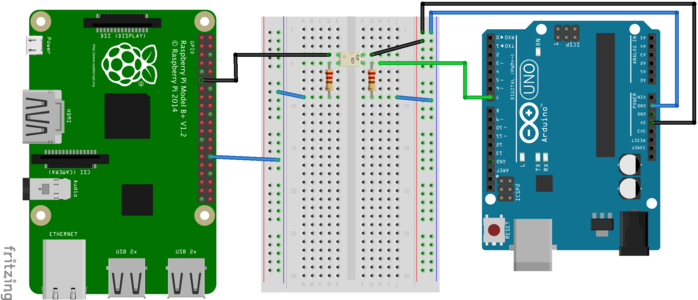
\includegraphics[width=0.8\textwidth]{bilder/aufbau.png}
 	\caption{Schematischer Aufbai}
	\label{aufbau}
\end{figure}
\noindent
Im eigentlichen Betrieb läuft der Simulator mit dem e.manager der Firma enerserve. Der e.manager erlaubt es Anlagen zu überwachen und den Verbrauch zu messen. Dies geschiet über diverse Schnittstellen, darunter auch die S0-Schnittstelle. Da der e.manager mit einer Spannung von 12 Volt betrieben wird, muss dieser galvanisch vom Raspberry PI getrennt werden, da dieser mit 5 Volt betrieben wird. Dies geschiet mit dem bereits erwähnten Optokoppler. Abbildung \ref{emanager} zeigt den Aufbau mit dem Raspberry PI und dem e.manager.
 \begin{figure}[H]
 	\centering
 	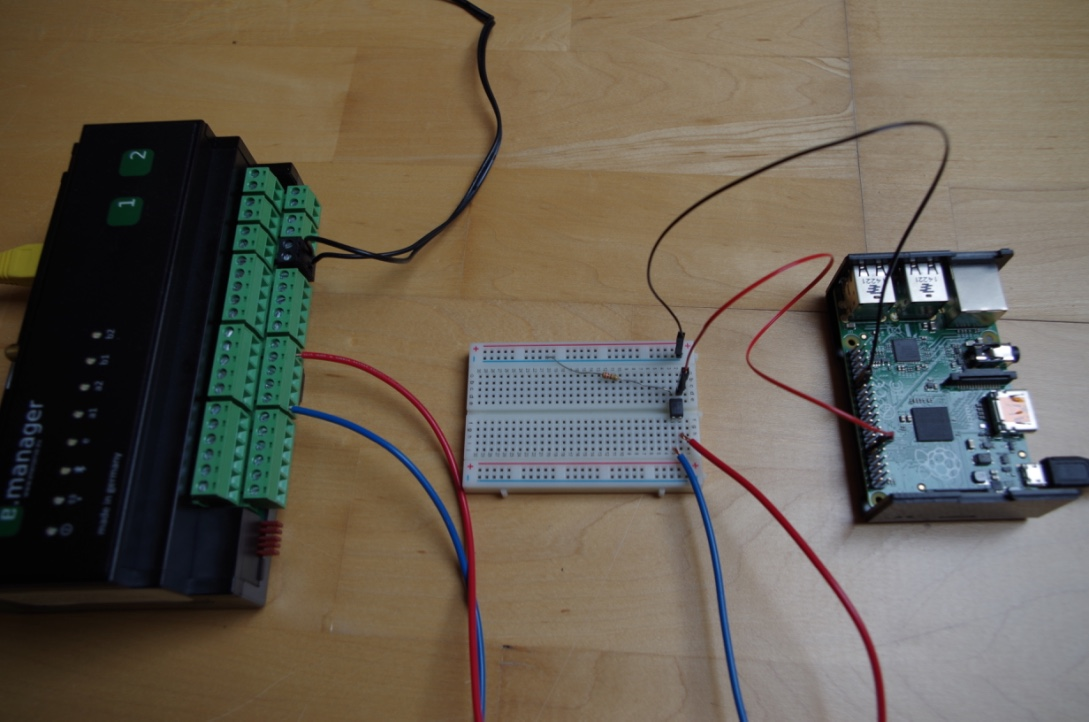
\includegraphics[width=0.8\textwidth]{bilder/aufbau.jpg}%TODO png ersetzen
 	\caption{Aufbau mit e.manager}
 	\label{emanager}
 \end{figure}
 \noindent
 Die ermittelten Daten des e.managers können über ein Webinterface abgerufen werden. Das Portal von enerserve (http://portal.enerserve.eu) erlaubt es dem Benutzer den Verlauf der einzelnen Geräte zu verfolgen. Neben Übersicht des akutellen Verbrauchs, liefert das Webinterface historische Daten abzufragen. Dabei wird zwischen Tages-, Monats- und Jahresansicht unterschieden. Weiterhin bietet das Interface eine Konfiguration der Anschlüsse.